\section{Electrical Design}
\label{sec:elec}

\subsection{Power}
A four-cell (4S) LiPo battery, \SI{14.8}{\volt} nominal,
supplies the boat through XT60 connectors and a power distribution board that
provides regulated rails for the servos and logic. The regulator outputs a 12V rail that powers out wind vane, and it outputs a 5V rail that powers the rudder and sail-tail servos as well as the STM32 board. Our battery capacity is rated for 1300 mAh.

The pack is monitored without a dedicated battery-monitor chip. Each
cumulative cell tap (cell 1, cells 1--2, cells 1--3, and the full pack) feeds
an analog-to-digital converter (ADC) channel through a divider with
$R_{\mathrm{top}} = \SI{82}{\kilo\ohm}$ and
$R_{\mathrm{bot}} = \SI{18}{\kilo\ohm}$, so the tap voltage is
\begin{equation}
V_{\mathrm{tap}} = V_{\mathrm{pin}}\,\frac{R_{\mathrm{top}} + R_{\mathrm{bot}}}{R_{\mathrm{bot}}}
               = 5.56\,V_{\mathrm{pin}} .
\label{eq:divider}
\end{equation}
By~\eqref{eq:divider}, a fully charged pack (\SI{16.8}{\volt}) appears as \SI{3.02}{\volt},
just inside the \SI{3.3}{\volt} ADC reference. A \SI{100}{\nano\farad}
capacitor across each divider forms a low-pass filter with a time constant of
about \SI{1.5}{\milli\second}. The firmware waits \SI{10}{\milli\second}
(about seven time constants) before converting and averages eight conversions per
channel in integer arithmetic. It samples at \SI{2}{\hertz} and averages the
last 20 readings, a ten-second window, before recovering each cell voltage by
subtracting adjacent taps. Pin PA1 was avoided because the Nucleo board ties it to the
Ethernet physical-layer clock, which injects noise.

\subsection{Sensors and Actuators}
Table~\ref{tab:elec} lists the components, the peripheral each uses, and its
sample rate. The BNO055 combines a three-axis accelerometer, gyroscope, and
magnetometer with onboard fusion~\cite{bno055}, so it supplies both the
IMU and magnetometer called for in the proposal;
it runs in its nine-degree-of-freedom (NDOF) fusion mode with stored
calibration offsets. The AS5600~\cite{as5600} measures sail angle. The BNO055 and AS5600 connect over separate inter-integrated circuit (I\textsuperscript{2}C) buses. The DFRobot wind
vane has an adapter that converts to a universal asynchronous receiver-transmitter (UART) signal for
the microcontroller. It is polled with a Modbus RTU ``read holding register''
request~\cite{modbus} protected by a 16-bit cyclic redundancy check (CRC) and reports apparent wind
direction in tenths of a degree. The u-blox NEO-6 GPS receiver streams National Marine Electronics Association (NMEA) 0183
sentences~\cite{nmea0183}; the firmware receives them by direct memory access
(DMA) with idle-line detection and parses the GGA sentence for position, fix
quality, and satellite count, and the RMC sentence for speed and course over
ground, which the tack planner uses. Position is marked valid only while the
most recent GGA sentence reported a fix.

Both servos are driven by pulse-width modulation (PWM) from timer TIM1 at \SI{50}{\hertz}, with pulse widths
from \SI{500}{\micro\second} to \SI{2500}{\micro\second} mapped linearly to
$\pm\SI{90}{\degree}$.

\begin{table}[!t]
\caption{Electronic Components and Interfaces}
\label{tab:elec}
\centering
\begin{tabular}{@{}p{0.2\columnwidth}p{0.36\columnwidth}p{0.32\columnwidth}@{}}
\toprule
Function & Component & Interface, rate \\
\midrule
Controller   & NUCLEO-H755ZI-Q (STM32H755) & -- \\
Orientation  & Bosch BNO055, NDOF mode & I\textsuperscript{2}C2, \SI{50}{\hertz} \\
Sail angle   & ams AS5600 12-bit encoder & I\textsuperscript{2}C1, \SI{10}{\hertz} \\
Wind         & DFRobot RS-485 wind vane, Modbus RTU & UART4 via RS-485 adapter, \SI{5}{\hertz} \\
Position     & u-blox NEO-6 GPS, NMEA GGA & UART7 + DMA, \SI{1}{\hertz} \\
Battery      & Four divider taps & ADC1, \SI{2}{\hertz} \\
Telemetry    & RFM95W (SX1276) LoRa & SPI1 on CM4, \SI{1}{\hertz} \\
Rudder       & DS3218MG 20 kg-cm servo & TIM1 PWM, \SI{50}{\hertz} \\
Tail         & MG90S 9G Servo & TIM1 PWM, \SI{50}{\hertz} \\
Debug        & ST-LINK virtual COM port & USART3, 115200 Bd \\
\bottomrule
\end{tabular}
\end{table}

\subsection{Communication Link}
The boat communicates with an elevated ground station over line of sight. The
team chose LoRa (long range) modulation~\cite{augustin2016} over Wi-Fi or
Bluetooth because the traffic is small and infrequent and because low power
consumption is a design priority. LoRa operates in the unlicensed industrial,
scientific, and medical (ISM) bands, at \SI{915}{\mega\hertz} in North
America. Sub-gigahertz signals reach farther than \SI{2.4}{\giga\hertz}
signals because they diffract more readily around obstacles and because
free-space path loss (FSPL) grows with frequency:
\begin{equation}
\mathrm{FSPL} = 20\log_{10} d + 20\log_{10} f + 20\log_{10}\!\left(\frac{4\pi}{c}\right),
\label{eq:fspl}
\end{equation}
with distance $d$ in meters, frequency $f$ in hertz, and $c$ the speed of
light. At \SI{1}{\kilo\meter}, \eqref{eq:fspl} gives \SI{91.7}{dB} at
\SI{915}{\mega\hertz} and \SI{100.0}{dB} at \SI{2.4}{\giga\hertz}, an
\SI{8.4}{dB} advantage that corresponds to about 2.6 times the range for the
same link budget.

The RFM95W module (Semtech SX1276 transceiver~\cite{sx1276}) is configured for
spreading factor (SF) 8, \SI{125}{\kilo\hertz} bandwidth (BW), coding rate (CR) 4/5,
explicit header, hardware CRC, and \SI{17}{dBm} output on the PA\_BOOST pin. The CM4 talks to the module over the serial peripheral interface (SPI).
The time on air of one packet follows from the symbol time
$T_s = 2^{\mathrm{SF}}/\mathrm{BW}$ and the payload symbol
count~\cite{sx1276}
\begin{multline}
n_{\mathrm{pl}} = 8 + \max\Bigl(\Bigl\lceil \tfrac{8L - 4\,\mathrm{SF} + 28 + 16\,\mathrm{CRC} - 20\,\mathrm{IH}}{4(\mathrm{SF} - 2\,\mathrm{DE})} \Bigr\rceil (\mathrm{CR}+4),\, 0\Bigr),\\
T_{\mathrm{air}} = (n_{\mathrm{pre}} + 4.25 + n_{\mathrm{pl}})\,T_s ,
\label{eq:airtime}
\end{multline}
where $L$ is the payload length in bytes, CRC $=1$, implicit header IH $=0$,
low-data-rate optimization DE $=0$, CR $=1$, and $n_{\mathrm{pre}} = 8$. Applying~\eqref{eq:airtime} to
the 78-byte telemetry frame of Section~\ref{sec:sw} gives $T_s =
\SI{2.048}{\milli\second}$, $n_{\mathrm{pl}} = 108$, and $T_{\mathrm{air}}
\approx \SI{246}{\milli\second}$. Sent once per second, telemetry occupies
about a quarter of the channel; the radio spends the remaining time listening
for commands.

\subsection{Packaging}
The electronics are mounted in a printed enclosure that drops into the aft
hatch (Fig.~\ref{fig:electronics}). The microcontroller board is mounted along
one wall, with the radio, GPS receiver, and orientation sensor on printed
standoffs. The BNO055 is mounted flat and fixed to the hull so that its axes
stay aligned with the boat's. External cables enter through compression
glands, and the antenna feed passes through a sealed SMA bulkhead connector to
the masthead antenna. Interconnections are made on a solderless
breadboard. A KiCad schematic for a custom carrier board around the STM32H755
was started, but the board is no longer planned, so the breadboard remains in
the vessel as built. Its solderless contacts are vulnerable to vibration and
corrosion on the water.

\begin{figure}[!t]
\centering
\subfloat[]{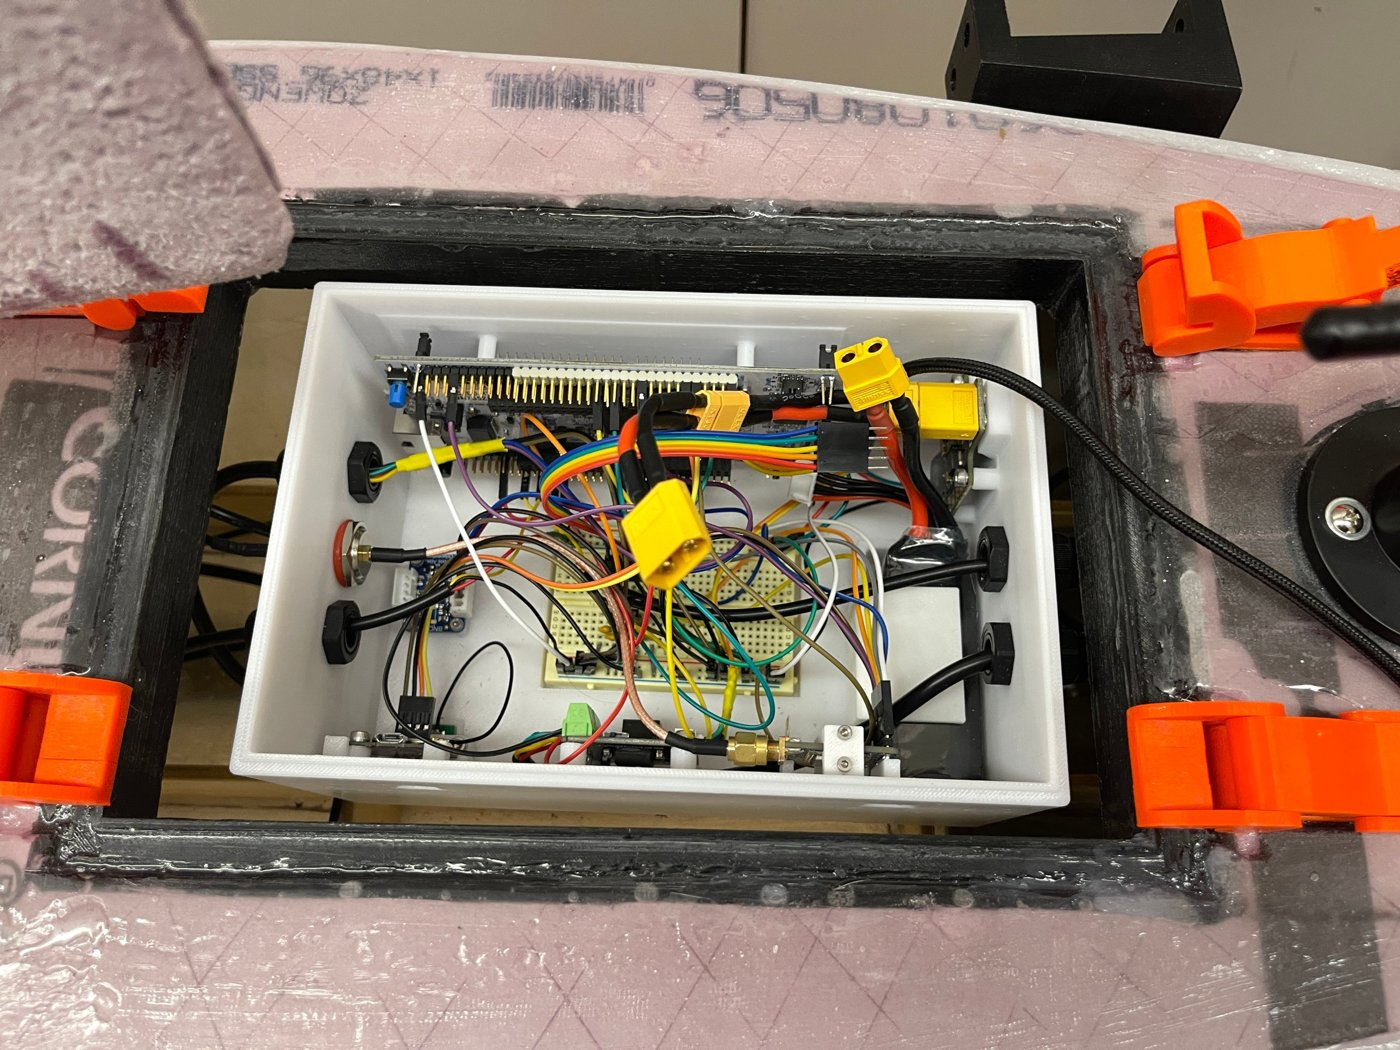
\includegraphics[width=0.56\columnwidth]{electronics_box}}
\hfil
\subfloat[]{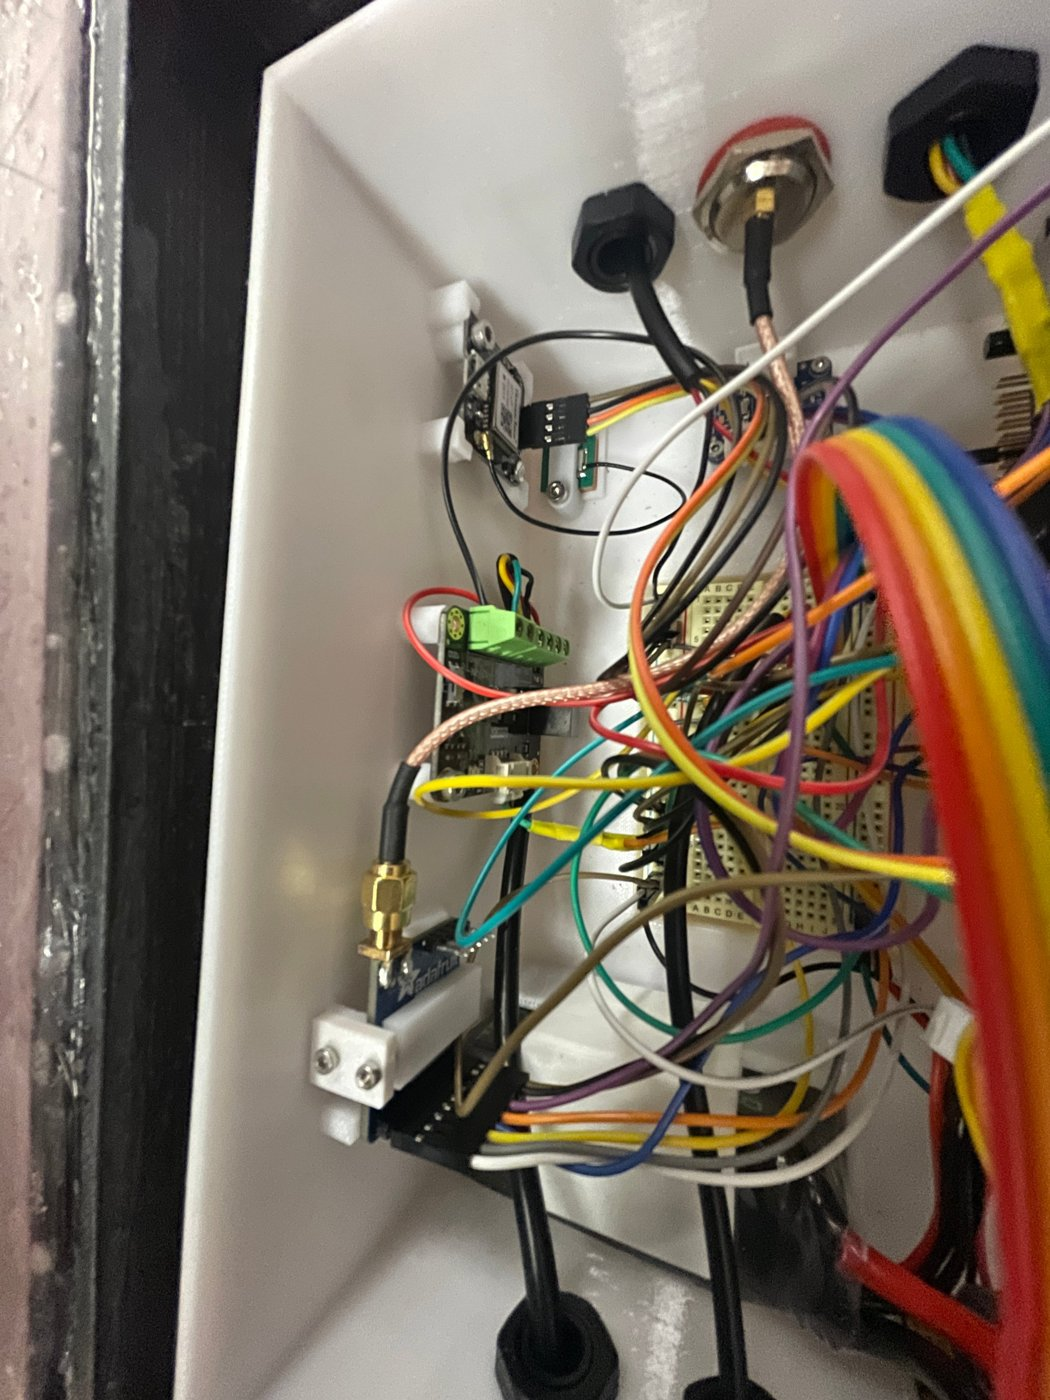
\includegraphics[width=0.33\columnwidth]{electronics_side}}
\caption{Electronics enclosure in the aft hatch. (a) Overview: NUCLEO-H755ZI-Q
board, power distribution board and XT60 connectors, breadboard, BNO055, and
cable glands. (b) Side wall: NEO-6 GPS module, RS-485 adapter for the wind vane, and LoRa
radio with its SMA feed to the bulkhead connector.}
\label{fig:electronics}
\end{figure}
